\iffalse
\let\negmedspace\undefined
\let\negthickspace\undefined
\documentclass[journal,12pt,twocolumn]{IEEEtran}
\usepackage{cite}
\usepackage{amsmath,amssymb,amsfonts,amsthm}
\usepackage{algorithmic}
\usepackage{graphicx}
\usepackage{textcomp}
\usepackage{xcolor}
\usepackage{txfonts}
\usepackage{listings}
\usepackage{enumitem}
\usepackage{mathtools}
\usepackage{gensymb}
\usepackage{comment}
\usepackage[breaklinks=true]{adjustbox}
\usepackage{tkz-euclide} 
\usepackage{listings}
\usepackage{gvv}                                        
\def\inputGnumericTable{}                                 
\usepackage[latin1]{inputenc}                                
\usepackage{color}                                            
\usepackage{array}                                            
\usepackage{longtable}                                       
\usepackage{calc}                                             
\usepackage{multirow}                                         
\usepackage{hhline}                                           
\usepackage{ifthen}                                           
\usepackage{lscape}

\newtheorem{theorem}{Theorem}[section]
\newtheorem{problem}{Problem}
\newtheorem{proposition}{Proposition}[section]
\newtheorem{lemma}{Lemma}[section]
\newtheorem{corollary}[theorem]{Corollary}
\newtheorem{example}{Example}[section]
\newtheorem{definition}[problem]{Definition}
\newcommand{\BEQA}{\begin{eqnarray}}
\newcommand{\EEQA}{\end{eqnarray}}
\newcommand{\define}{\stackrel{\triangle}{=}}
\theoremstyle{remark}
\newtheorem{rem}{Remark}

\begin{document}
\bibliographystyle{IEEEtran}

\vspace{3cm}

\title{}
\author{EE23BTECH11047 - Deepakreddy P
}
\maketitle

\noindent \textbf{17} \quad 
If a, b, c, d are in G.P, prove that 
$ \brak{a^{n} + b^{n}},\brak{b^{n} + c^{n}},\brak{c^{n} + d^{n}} $ are in G.P \\
\solution
\fi


\begin{center}
    \begin{table}[ht]
        \setlength{\arrayrulewidth}{0.3mm}
\setlength{\tabcolsep}{12pt}
\renewcommand{\arraystretch}{1.5}


\begin{center}
\caption{Input Parameters}
\begin{tabular}{|c|c|}

\hline
 {Symbol}&{Remarks}\\
\hline
$x(0) $ & $a$ \\
\hline
$x(1) $ & $b$ \\
\hline
$x(2) $ & $c$ \\
\hline
$x(3) $ & $d$ \\
\hline
$r$ & ratio of G.P a,b,c....\\
\hline
$r_1$ & ratio of G.P $a^n + b^n,b^n + c^n,....$\\
\hline
$X(z)$ & z transform of G.P a,b,c....\\
\hline
$Y(z)$ & z transform of G.P $a^n + b^n,b^n + c^n,....$\\
\hline

\end{tabular}
\label{Table:11.9.5.17.3}
\end{center}

    \end{table}
\end{center}

From \tabref{Table:11.9.5.17.3}

\begin{align}   
r=\frac{b}{a} = \frac{c}{b}= \frac{d}{c} \label{eq:eq.11.9.5.17.1}
\end{align}

From eq \eqref{eq:eq.11.9.5.17.1}

\begin{align}
\frac{b^n + c^n}{a^n + b^n}
&= \frac{\brak{ar}^n + \brak{ar^2}^n}{\brak{a}^n + \brak{ar}^n}\\
&= \frac{a^n r^n \brak{1+ r^n}}{a^n \brak{1 + r^n}}\\
&= r^n \\
\frac{c^n + d^n}{b^n + c^n}&= \frac{\brak{ar^2}^n + \brak{ar^3}^n}{\brak{ar}^n + \brak{ar^2}^n}\\
&= \frac{a^n r^{2n} \brak{1 + r^n}}{a^n r^n \brak{1 + r^n}}\\
%&= \frac{r^n \brak{\brak{ar}^n + \brak{ar^2}^n}}{r^n \brak{\brak{a}^n + \brak{ar}^n}}
&= r^n \\
\frac{b^n + c^n}{a^n + b^n} &= \frac{c^n + d^n}{b^n + c^n}
\end{align}
Hence proved they are in in G.P\\

\begin{align}
    x\brak{n} &= a\brak{\frac{b}{a}}^{n} u\brak{n}\\
    X\brak{z} &= \frac{a}{1-\brak{\frac{b}{a}} z^{-1}}, \quad \abs{z}>\abs{\frac{b}{a}}
\end{align}

\begin{align}   
r_1=\frac{b^n + c^n}{a^n + b^n} = \frac{c^n + d^n}{b^n + c^n} \label{eq:eq.11.9.5.17.2}
\end{align}

From eq \eqref{eq:eq.11.9.5.17.2}

\begin{align}
    y\brak{n} &= \brak{a^n + b^n} \brak{\frac{b^n + c^n}{a^n + b^n}}^{n} u\brak{n}\\
    Y\brak{z} &= \frac{a^n + b^n}{1-\brak{\frac{b^n + c^n}{a^n + b^n}} z^{-1}}, \quad \abs{z}>\abs{\frac{b^n + c^n}{a^n + b^n}}
\end{align}


\begin{figure}[ht]
   \centering
   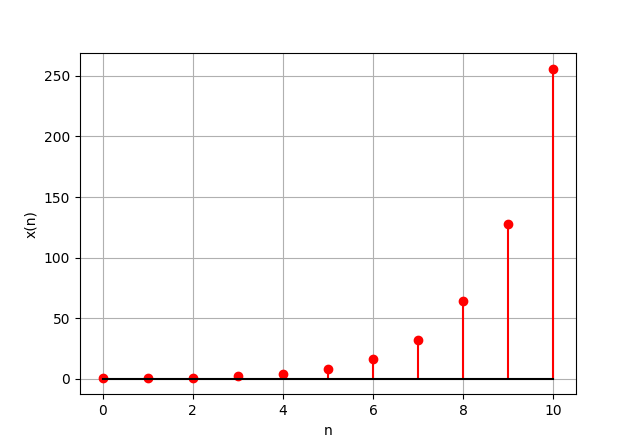
\includegraphics[width=0.8\columnwidth]{ncert-maths/11/9/5/17/figs/gp1.png}
   \caption{Stem Plot of $x(n) = (0.25) 2^n u(n)$, $a= 0.25, r=2$}
\end{figure}

\begin{figure}[ht]
   \centering
   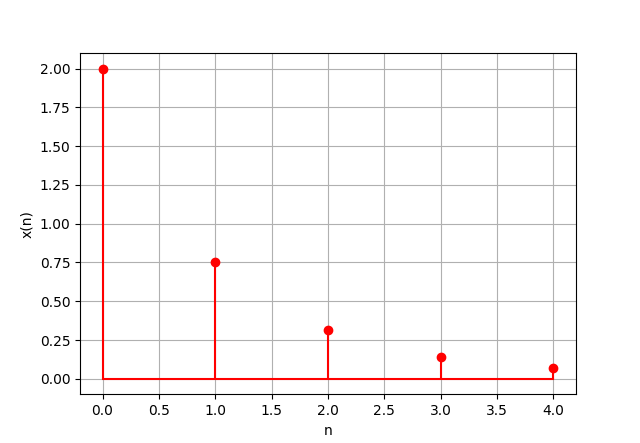
\includegraphics[width=0.8\columnwidth]{ncert-maths/11/9/5/17/figs/gp2.png}
   \caption{Stem Plot of $x(n) = \brak{0.25^n + 0.5^n} u(n)$, $a=0.25, b=0.5$}
\end{figure}

%\end{document}
